\section{Typisches Aussehen einer Evolutionsstrategie}
%1. Obwohl viel Variation, erkannte Rechenberg Abschnitte die häufig wiederzufinden sind
Evolutionsstrategien können einen sehr hohen Grad an Variation aufweisen. Je nach Aufgabengebiet unterscheiden sich die Verfahren stark.
Rechenberg konnte allerdings Verfahrensabschnitte benennen, aus denen sich typischerweise Evolutionsstrategien zusammensetzen.
Diese Verfahrensabschnitte bilden die Rechenbergsche Grafik-Notation \cite[S.144-146]{schoeneburg}. In diesem Kapitel wird mit Hilfe der Rechenbergschen Grafik-Notation das typische Aussehen einer Evolutionsstrategie erläutert.

\subsection{Rechenbergsche Grafik-Notation}
%2. Die Rechenbergnotation erklären
Die  Rechenbergschen Grafik-Notation orientiert sich an Spielkarten und kommt mit lediglich 10 verschiedenen Symbolen aus.
Die gesamte Rechenbergsche Grafik-Notation ist in Abbildung \ref{fig:rechenberg} zu sehen. Abläufe, die in einer natürlichen Evolution stattfinden, finden sich in dieser Notation wieder.
Die Komplexität der Evolutionsstrategien wird durch deren Kombination erreicht.\\
Die grundlegende Einheit in dieser Notation ist das Individuum. Dieses wird mit einer Spielkarte (\ref{fig:individuum}) symbolisiert. Die schwarzen Punkte auf der Karte sollen dabei die Chromosomen darstellen.
Eine Population setzt sich aus mehreren Individuen zusammen. Daher wählte Rechenberg einen Stapel (\ref{fig:population}) an Spielkarten für dessen Darstellung. Zur Verarbeitung der Individuen und der Populationen definierte Rechenberg acht weitere Symbole.
Für die Verarbeitung von Populationen stehen Methoden bereit, mit denen eine Teilmenge an Individuen ausgewählt werden kann. Dazu gibt es die gleichverteile Auswahl \ref{fig:auswahl_gleichverteilt} und die Auswahl nach einer Qualitätsfunktion \ref{fig:auswahl_qualitaetsfunktion}.
Der Kreis um die Population soll eine Urne symbolisieren, aus der Individuen gezogen werden. Bei der gleichverteilten Auswahl hat jedes Individuum die gleiche Wahrscheinlichkeit aus der Urne gezogen zu werden. Bei der Auswahl nach einer Qualitätsfunktion entscheidet die Qualität der Individuen über die Wahrscheinlichkeit, dass diese Ausgwählt werden.
Je höher die Qualität des Individuum, desto höher die Wahrscheinlichkeit. Auch das Verwenden von isolierten Populationen ist mit der Rechenbergschen Grafik-Notation möglich. Dafür gibt das Populationssymbol \ref{fig:population_isoliert}, welches mit einem Stacheldraht eingegrenzt ist. Dieses Symbol kann hilfreich sein, wenn man mehrere voneinander isolierte Populationen erstellen will, welche sich unabhängig voneinander entwickeln sollen.\\
Alle weiteren Notationssymbole sind Funktionen, die auf einzelne Individuen angewendet werden. Um ein Individuum zu duplizieren, wird das Symbol \ref{fig:duplikation} verwendet. Soll das duplizierte Individuum mutieren, so ist das Symbol \ref{fig:mutation} zu verwenden. Zeigt, wie auf dem Symbol \ref{fig:bewertung}, ein Pfeil mit einem Q auf ein Individuum, so wird eine Qualitätsfunktion auf das Individuum angewendet. Damit auch die Fortpflanzung mehrerer Individuen zu einem neuen Individuum möglich ist, gibt es eigens das Notationssymbol \ref{fig:rekombination} für die Rekombination. Rekombination bedeutet, dass durch eine Kombination der Elternchromosome ein neues Kindindividuum erzeugt wird.
Es kann auch notwendig sein, die genotypischen Merkmale in phänotypische Merkmale umzuwandeln. Dies ist dann notwendig, wenn über die Geninformationen nicht direkt eine Aussage über die Qualität des Individuums getroffen werden kann. In diesen Fällen müssen die Merkmale, die sich aus den Geninformationen ergeben in einer Funktion berechnet werden. Dieses Umwandeln wird mit dem Symbol der phänotypischen Realisation \ref{fig:phaenotypische_realisation} dargestellt.

\begin{figure}[!htb]
\begin{subfigure}{.3\textwidth}
	\centering
	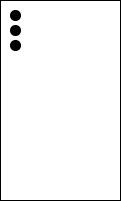
\includegraphics[width=.4\linewidth]{img/rechenberg_notation/individuum.png}
	\caption{Individuum}
	\label{fig:individuum}
\end{subfigure}
\begin{subfigure}{.3\textwidth}
	\centering
	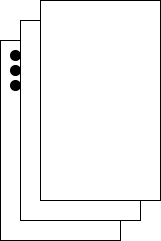
\includegraphics[width=.5\linewidth]{img/rechenberg_notation/population.png}
	\caption{Population}
	\label{fig:population}
\end{subfigure}
\begin{subfigure}{.3\textwidth}
	\centering
	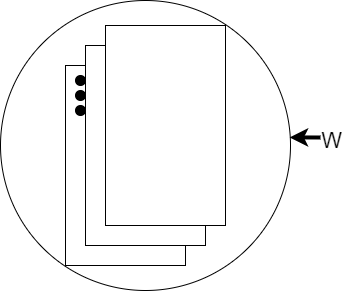
\includegraphics[width=.7\linewidth]{img/rechenberg_notation/auswahl_gleichverteilt.png}
	\caption{Gleichverteilte Auswahl}
	\label{fig:auswahl_gleichverteilt}
\end{subfigure}

\begin{subfigure}{.3\textwidth}
	\centering
	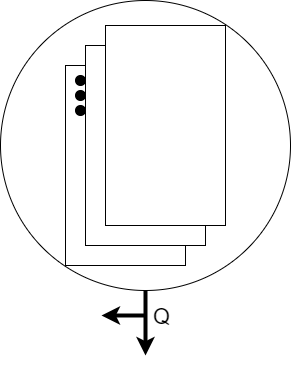
\includegraphics[width=.7\linewidth]{img/rechenberg_notation/auswahl_qualitaetsfunktion.png}
	\caption{Auswahl mit einer Qualitätsfunktion}
	\label{fig:auswahl_qualitaetsfunktion}
\end{subfigure}
\begin{subfigure}{.3\textwidth}
	\centering
	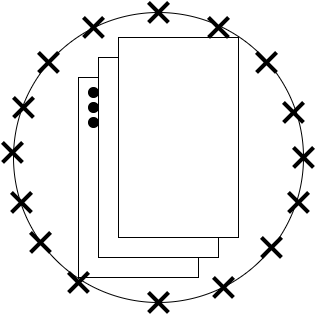
\includegraphics[width=.7\linewidth]{img/rechenberg_notation/population_isoliert.png}
	\caption{Isolierte Population}
	\label{fig:population_isoliert}
\end{subfigure}
\begin{subfigure}{.3\textwidth}
	\centering
	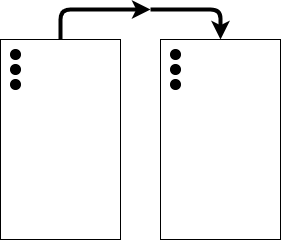
\includegraphics[width=.7\linewidth]{img/rechenberg_notation/duplikation.png}
	\caption{Duplikation}
	\label{fig:duplikation}
\end{subfigure}

\begin{subfigure}{.3\textwidth}
	\centering
	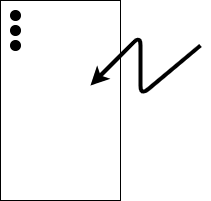
\includegraphics[width=.7\linewidth]{img/rechenberg_notation/mutation.png}
	\caption{Mutation}
	\label{fig:mutation}
\end{subfigure}
\begin{subfigure}{.3\textwidth}
	\centering
	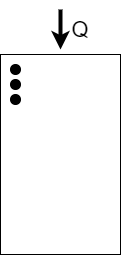
\includegraphics[width=.4\linewidth]{img/rechenberg_notation/bewertung.png}
	\caption{Bewertung}
	\label{fig:bewertung}
\end{subfigure}
\begin{subfigure}{.3\textwidth}
	\centering
	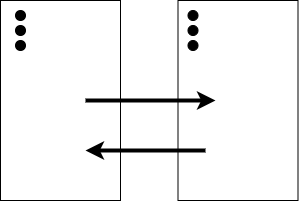
\includegraphics[width=.7\linewidth]{img/rechenberg_notation/rekombination.png}
	\caption{Rekombination}
	\label{fig:rekombination}
\end{subfigure}

\begin{subfigure}{.3\textwidth}
	\centering
	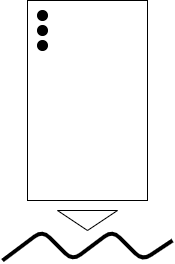
\includegraphics[width=.5\linewidth]{img/rechenberg_notation/phaenotypische_realisation.png}
	\caption{Phänotypische Realisation}
	\label{fig:phaenotypische_realisation}
\end{subfigure}
\caption{Rechenbergsche Grafik-Notation \cite[S. 145]{schoeneburg}.}
\label{fig:rechenberg}
\end{figure}


% 3. Typische Reihenfolge der Abschnitte kurz zeigen. Aber auch klar machen das das ganze extrem variieren kann
\subsection{Aufbau einer Evolutionsstrategie}

Die Rechenbergsche Grafik-Notation wird im folgenden zur Modellierung des Aufbaus von Evolutionsstrategien verwendet. In Abbildung \ref{fig:flowchart_es} ist ein Flussdiagramm zu sehen, das den Ablauf einer Evolutionsstrategie abstrakt darstellt.
Zu Beginn wird eine Startpopulation gebildet. Für diese Population können die Chromosome der einzelnen Individuen zufällig gewählt werden. Aus dieser Population wird anschließend eine Teilmenge gebildet. Diese Teilmenge kann als Elternpopulation bezeichnet werden, denn die Nachkommen werden aus diesen Individuen erzeugt. Bei den Evolutionsstrategien hat jedes Individuum die selbe Wahrscheinlichkeit für die Elternpopulation ausgewählt zu werden \cite[S.220]{schoeneburg}. Eine Auswahl über deren Qualität findet nicht statt. Die Nachkommen der Elternpopulation werden erzeugt, indem die Eltern dupliziert werden. Die Generation der Nachkommen kann auch durch eine Kombination der Chromosome von mehreren Elternindividuen gebildet werden. Anschließend wird zu einem gewissen Prozentteil das Chromosom der Individuen mutiert. 
Nach der Mutation haben sich aus der Elternpopulation eine Nachkommenpopulation gebildet. Aus der Startpopulation und der Nachkommenpopulation wird anschließend über eine Selektion eine neue Population erzeugt. Die Selektion beruht, anders als bei der Bildung der Elternpopulation, auf Grundlage einer Qualitätsfunktion.
Bei der Auswahl der Individuen gibt es verschiedene Ansätze, die im Laufe dieser Ausarbeitung näher beschrieben werden. Genügt die Qualität der Population noch nicht den gewünschten Ansprüchen, so kann kann die gebildete Population für einen weiteren Evolutionsschritt verwendet werden.
Das grundlegende Verfahren ist im Pseudocode \ref{lst:es} übersichtlich aufgeführt. Die wenigen notwendigen Schritte aus denen sich Evolutionsstrategien zusammensetzen verdeutlichen, dass es Rechenberg nicht darum ging die Evolution perfekt nachzubilden, sondern diese lediglich als Anfangspunkt einer technischen Umsetzung zu betrachten. Aus diesem Grund sind in den nächsten Kapiteln dieser Ausarbeitung Evolutionsstrategien zu sehen, die sich zwar an der natürlichen Evolution orientieren, diese aber nicht versuchen realitätsnah abzubilden.
\begin{lstlisting}[caption={Grundlegende Evolutionsstrategie}, firstnumber=1, captionpos=b, label=lst:es]
algorithm ES()
	iterationsLimit <- x $\in \mathbb{N}$
	wunschqualitaet <- y $\in \mathbb{R}$
	generationszaehler <- 0
	population <- baue_population()
	while qualitaet(population) < wunschqualitaet or generationszaehler < iterationslimit
		generationszähler <- generationszähler + 1
		eltern <- elternSelektion(population)
		kinder <- duplikation(eltern) // oder: rekombination(eltern)
		kinder <- mutation(kinder)
		population <- selektion(eltern + kinder, size(population), qualitaet)
	loesung <- bestenSelektion(population)
\end{lstlisting}

\begin{figure}[!htb]
	\centering
	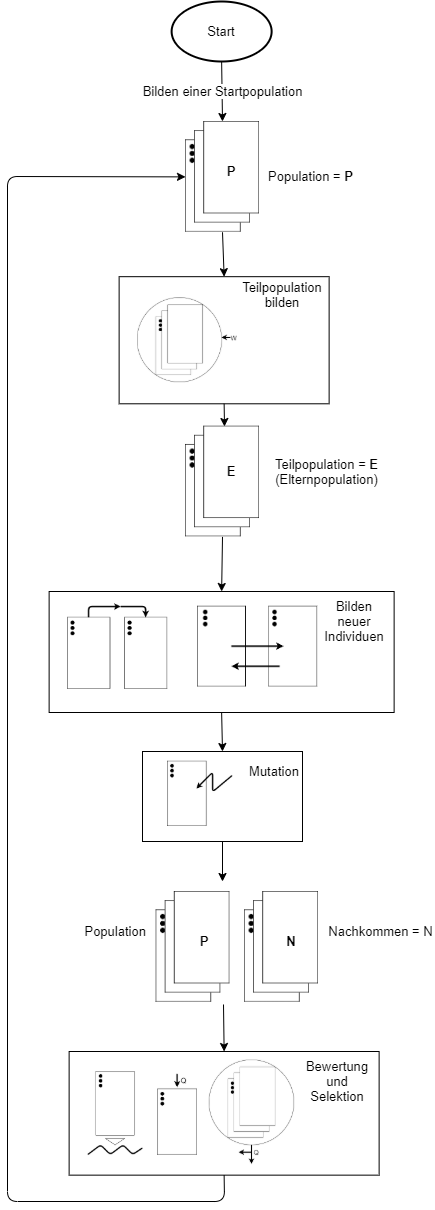
\includegraphics[height=\textheight, keepaspectratio]{img/typisches_aussehen/es_grafik.png}
	\caption{Flussdiagramm einer Evolutionsstrategie}
	\label{fig:flowchart_es}
\end{figure}



